\section{Clinical Examples}

\subsection{Susceptibility Weighted Imaging (SWI) of the Brain}

SWI is an MR technique used to enhance microhemorrhage and calcification in the brain.  This sequence exploits distortion of the MR field by paramagnetic (e.g., deoxyhemoglobin) and diamagnetic (e.g., dystrophic calcification) compounds, requiring the combination of magnitude and unwrapped phase images.  An example of a wrapped phase image obtained from an SWI sequence is shown in Figure~\ref{fig:SWI}.  The image is an axial slice taken through the brain.

\begin{figure}[h]
\center

\includegraphics[width=0.24\textwidth]{images/input/wrapped_swi.png}

\itkcaption[SWI of the Brain]{Wrapped phase data from SWI of the brain.}
\label{fig:SWI}
\end{figure}

The \code{itk::PhaseResidueImageFilter}, \code{itk::PhaseDerivativeVarianceImageFilter}, and \code{itk::HelmholtzDecompositionImageFilter} classes are demonstrated for the SWI data in Figure~\ref{fig:Exploring_SWI_Data}.  The residues are almost entirely restricted to the region outside the skull.  The Helmholtz decomposition shows that, as expected, most of the information in the low-quality, residue-rich region outside the skull is due to the rotational contribution, whereas most of the upward spike in phase in the anterior brain tissue is due to the irrotational contribution.  The phase derivative variance image shows high quality phase data within the brain tissue and low quality data otherwise.

\begin{figure}[h]
\center
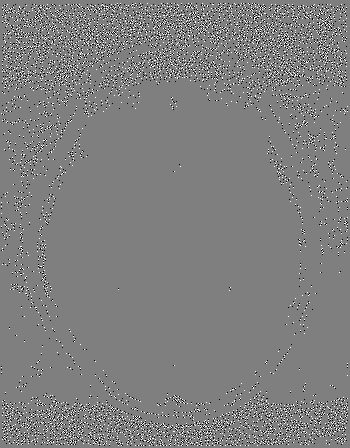
\includegraphics[width=0.24\textwidth]{images/swi/03a_residue.png}

\includegraphics[width=0.24\textwidth]{images/swi/03b_irrotational.png}
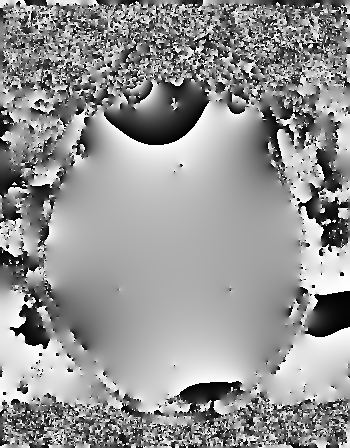
\includegraphics[width=0.24\textwidth]{images/swi/03c_rotational.png}

\includegraphics[width=0.24\textwidth]{images/swi/03d_quality.png}

\itkcaption[Exploring_SWI_Data]{Phase data from susceptibility weighted imaging of the brain.  From left to right: residues; irrotational component; rotational component; normalized phase derivative variance.}
\label{fig:Exploring_SWI_Data}
\end{figure}


\begin{figure}
\center

\includegraphics[width=0.32\textwidth]{images/input/wrapped_swi.png}

\includegraphics[width=0.32\textwidth]{images/swi/03e_qg_unwrap.png}

\includegraphics[width=0.32\textwidth]{images/swi/03f_dct_unwrap.png}

\itkcaption[Unwrapped Susceptibility Data]{Phase data from susceptibility weighted imaging of the brain.  Presented are the original image (left), the result of the quality-guided phase unwrapping algorithm (\code{itk:QualityGuidedPhaseUnwrappingImageFilter}, center), and of the DCT phase unwrapping algorithm (\code{itk:DCTPhaseUnwrappingImageFilter}, right).}
\label{fig:SWI_Unwrap}
\end{figure}

We now present the results of the Quality-Guided and DCT phase unwrapping algorithms (Figure~\ref{fig:SWI_Unwrap}).  The quality-guided approach (center) appears to correctly unwrap through the vast majority of the brain matter.  Upon close inspection, however, small areas of `roughness' are noted in regions of the brain matter closely correlating with residue pairs and clusters in the original image, presumably due to local noise (Figure~\ref{fig:SWI_Quality_Inset}).  The minimum $L^2$-norm approach gives a smooth result throughout.


\begin{figure}[h]
\center

\begin{tikzpicture}
    \node[anchor=south west,inner sep=0] (image) at (0,0) {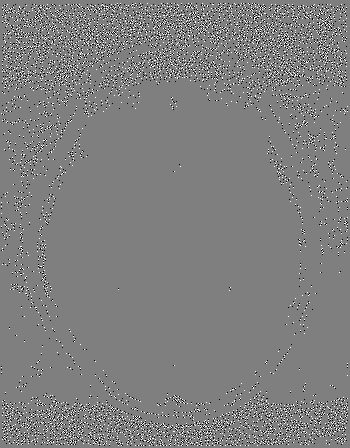
\includegraphics[trim = 70px 260px 70px 65px, clip, width=0.49 \textwidth]{images/swi/03a_residue.png}};
    \begin{scope}[x={(image.south east)},y={(image.north west)}]
        \draw [red] (0.5,0.675) ellipse (0.75cm and 0.5cm);
        \draw [red] (0.5,0.15) ellipse (0.75cm and 0.5cm);
    \end{scope}
\end{tikzpicture}

\begin{tikzpicture}
    \node[anchor=south west,inner sep=0] (image) at (0,0) {
\includegraphics[trim = 70px 260px 70px 65px, clip, width=0.49 \textwidth]{images/swi/03e_qg_unwrap.png}};
    \begin{scope}[x={(image.south east)},y={(image.north west)}]
        \draw [red] (0.5,0.675) ellipse (0.75cm and 0.5cm);
        \draw [red] (0.5,0.15) ellipse (0.75cm and 0.5cm);
    \end{scope}
\end{tikzpicture}


\itkcaption[SWI_Quality_Inset]{ Inset of the SWI residue (upper) and quality-guided phase unwrapped (lower) images.  Note the regions of minor discontinuity in the unwrapped image in regions corresponding to pairs/clusters of residues. }
\label{fig:SWI_Quality_Inset}
\end{figure}

A cross-section through the vertical centerline of the image is plotted in Figure~\ref{fig:SWI_Congruence}.  The quality-guided approach gives a congruent result throughout.  The DCT algorithm follows the gradient closely, but underestimates the phase.

\begin{figure}[h]
\center

\begin{tikzpicture}
    \node[anchor=south west,inner sep=0] (image) at (0,0) {
\includegraphics[width=0.28\textwidth]{images/input/wrapped_swi.png}};
    \begin{scope}[x={(image.south east)},y={(image.north west)}]
        \draw[red,ultra thick] (0.5,0) -- (0.5,1);
    \end{scope}
\end{tikzpicture}
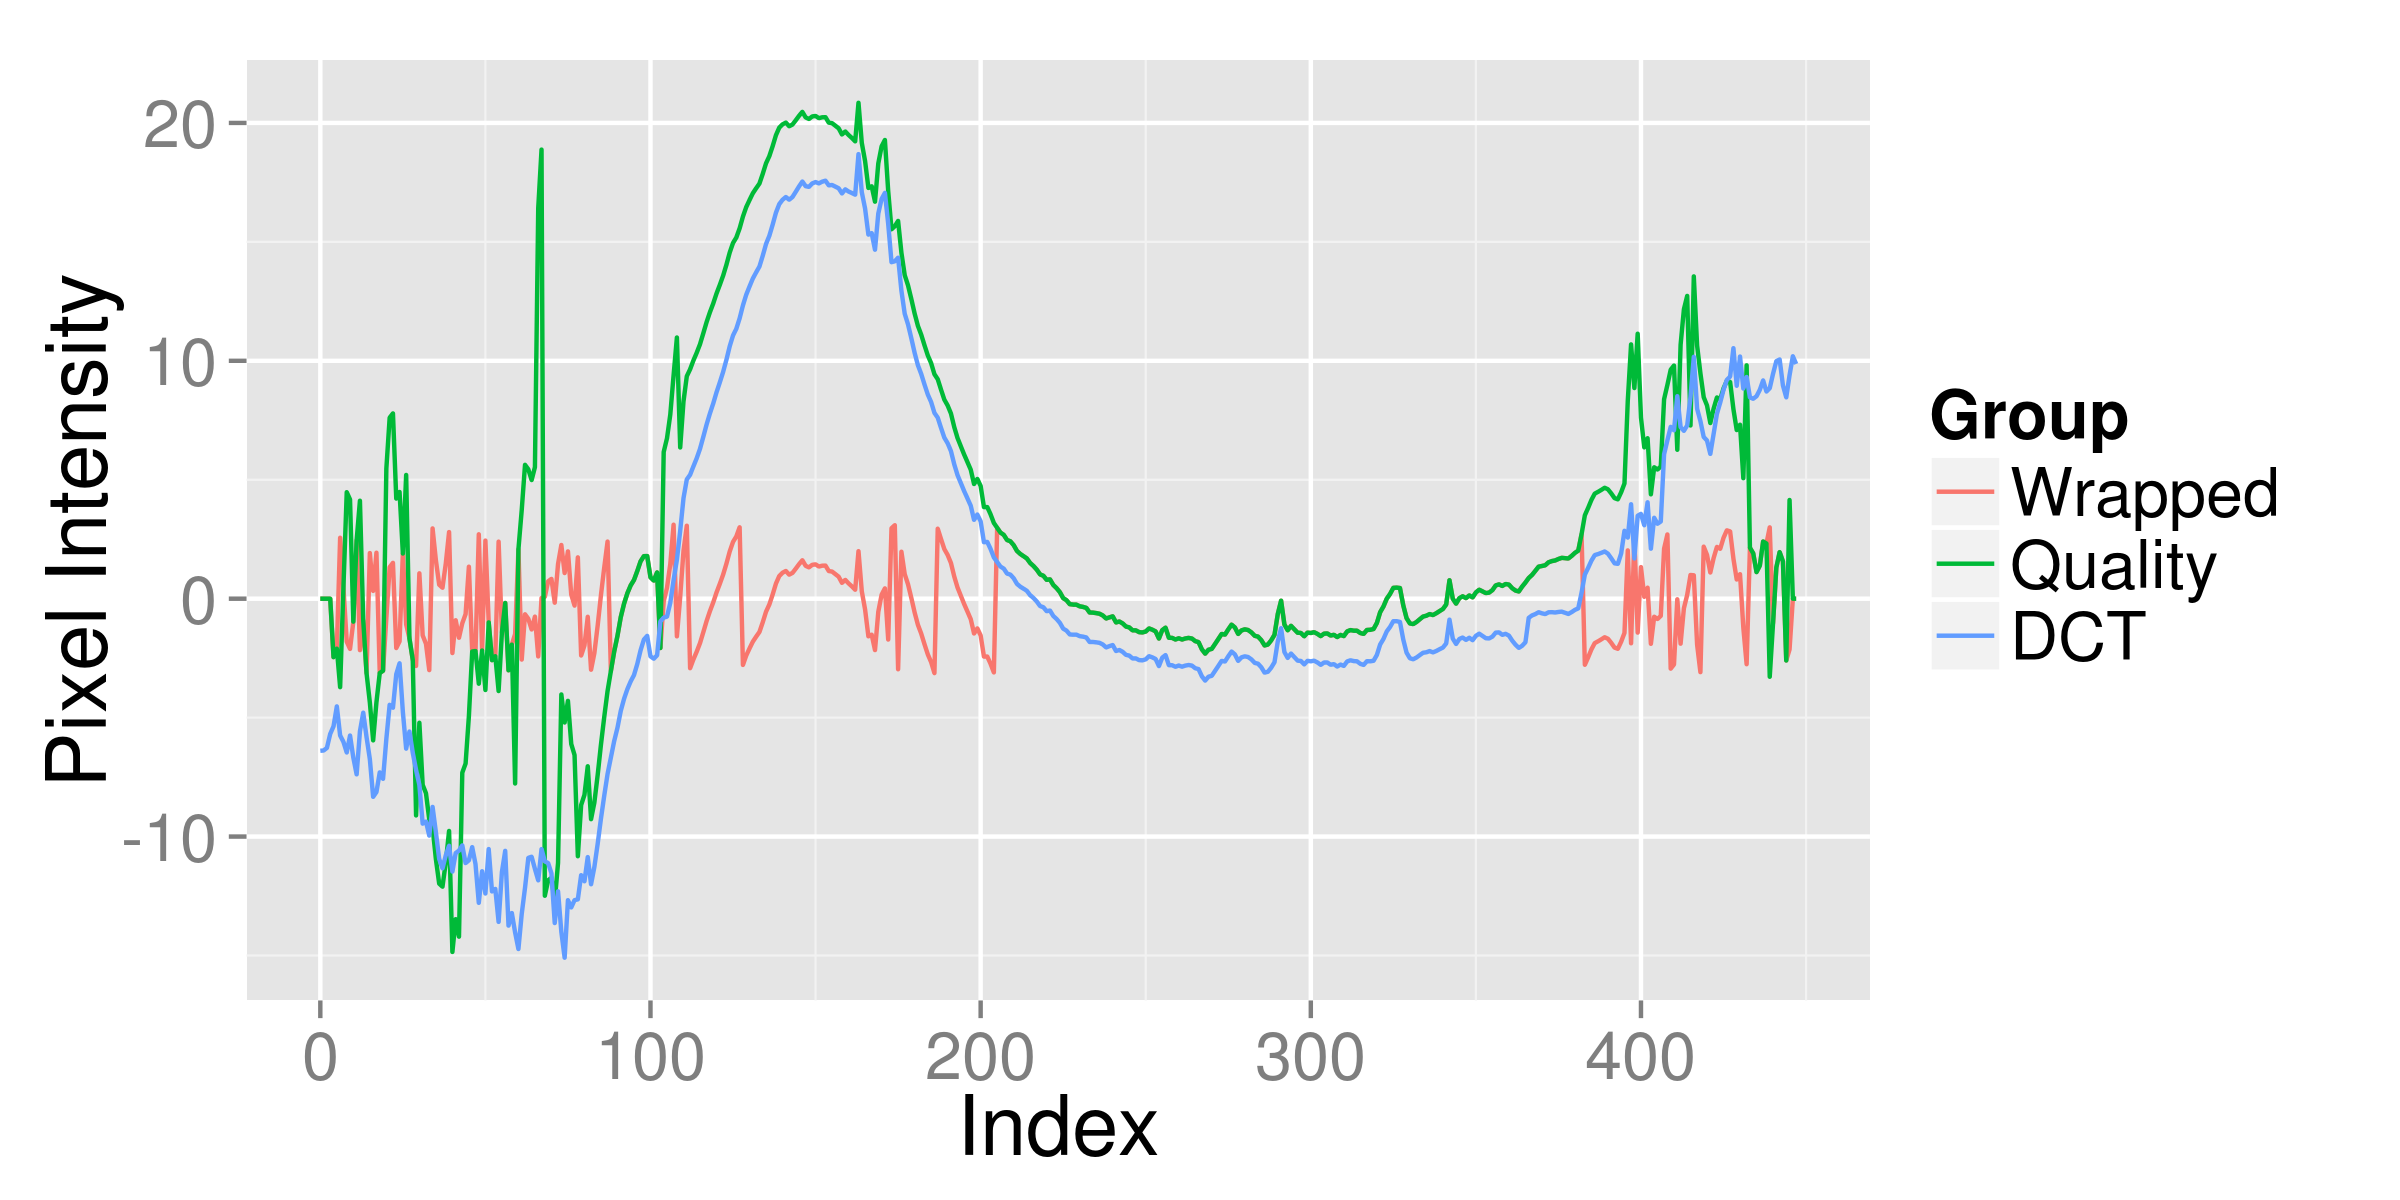
\includegraphics[width=0.71\textwidth]{images/swi/congruence.png}
\itkcaption[SWI_Congruence]{Congruence in SWI Data.  The pixel intensities from the vertical centerline of the SWI image are plotted for the unwrapped and original SWI data.  Note that the quality-guided approach is congruent throughout, but contains a discontinuity.  The DCT approach is smooth throughout, but is not congruent.}
\label{fig:SWI_Congruence}
\end{figure}

\newpage
\subsection{Harmonic Phase (HARP) Imaging of the Heart}

Spatial modulation of magnetization (SPAMM) is an MRI pulse sequence which modulates the signal magnitude in a periodic fashion across the plane of the image, resulting in lines of decreased signal \cite{Axel1989}.  The phase of this magnetude modulation is a material property of the tissue, and as such remains constant over time and with movement.  Therefore, tag lines laid down in the heart at end diastole will deform along with the heart during contraction, and so can be used to visualize cardiac deformation (Figure~\ref{fig:SPAMM}).

\begin{figure}[h]
\center
% left bottom right top
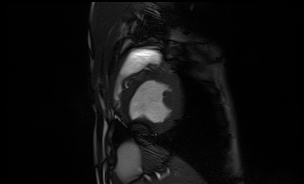
\includegraphics[trim = 100px 40px 110px 34px, clip, width=0.24\textwidth]{images/canine/ssfp_ed.png}

\includegraphics[trim = 100px 50px 110px 30px, clip, width=0.24\textwidth]{images/canine/spamm_ed.png}
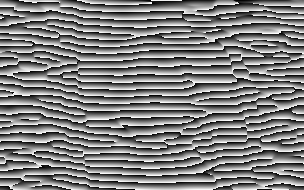
\includegraphics[trim = 100px 50px 110px 30px, clip, width=0.24\textwidth]{images/input/wrapped_harp_ed.png} \\
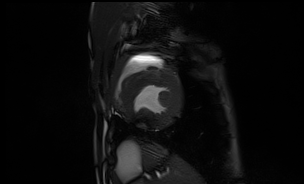
\includegraphics[trim = 100px 40px 110px 34px, clip, width=0.24\textwidth]{images/canine/ssfp_es.png}

\includegraphics[trim = 100px 50px 110px 30px, clip, width=0.24\textwidth]{images/canine/spamm_es.png}
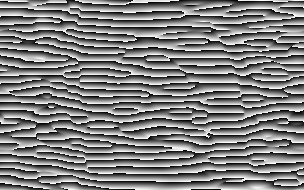
\includegraphics[trim = 100px 50px 110px 30px, clip, width=0.24\textwidth]{images/input/wrapped_harp.png}

\itkcaption[SPAMM]{Balanced steady state free precession (SSFP) images (left) are shown alongside corresponding tagged SPAMM (center) and HARP (right) images in a canine subject.  Shown are short axis, mid-ventricular images.  The upper panels were acquired at end diastole (no contraction); the lower panels were acquired at end systole (maximal contraction).  Note that circumferential shortening and radial thickening of the myocardium is apparent by observing the deformation of the tag lines.}
\label{fig:SPAMM}
\end{figure}

Harmonic phase analysis is an automated technique for calculating strain from tagged MR images \cite{Osman1999a}.  Cardiac strain is calculated from ``HARP'' images, which are the result of filtering in the Fourier domain.  Many versions of this algorithm require that these images be unwrapped prior to strain calculation \cite{Venkatesh2010, Venkatesh2011}.  SSFP, SPAMM, and HARP images at end systole and end diastole are shown in Figure~\ref{fig:SPAMM}.

The \code{itk::PhaseResidueImageFilter}, \code{itk::PhaseDerivativeVarianceImageFilter}, and \code{itk::HelmholtzDecompositionImageFilter} classes are demonstrated for the HARP data in Figure~\ref{fig:Exploring_HARP_Data}.

\begin{figure}[h]
\center
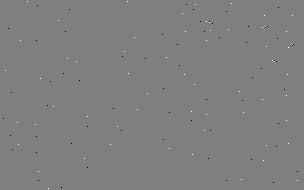
\includegraphics[trim = 100px 50px 110px 30px, clip, width=0.24\textwidth]{images/harp/03a_residue.png}
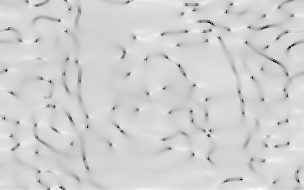
\includegraphics[trim = 100px 50px 110px 30px, clip, width=0.24\textwidth]{images/harp/03d_quality.png}

\includegraphics[trim = 100px 50px 110px 30px, clip, width=0.24\textwidth]{images/harp/03b_irrotational.png}
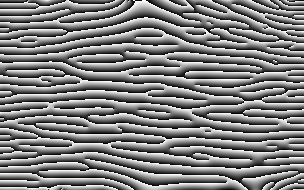
\includegraphics[trim = 100px 50px 110px 30px, clip, width=0.24\textwidth]{images/harp/03c_rotational.png}

\itkcaption[Exploring_HARP_Data]{Phase data from HARP imaging of the heart.  From left to right: residues, phase derivative variance, irrotational component, and rotational component.}
\label{fig:Exploring_HARP_Data}
\end{figure}

We now present the results of the Quality-Guided and DCT phase unwrapping algorithms (Figure~\ref{fig:HARP_Unwrap}).  From the unwrapped image it is clear that the quality-guided approach gives an unsatisfactory result, with phase wraps passing through the myocardial wall.  The result of the DCT approach is smooth, but otherwise difficult to evaluate by looking at the image directly.

\begin{figure}[h]
\center
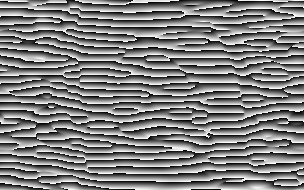
\includegraphics[trim = 100px 50px 110px 30px, clip, width=0.32\textwidth]{images/input/wrapped_harp.png}

\includegraphics[trim = 100px 50px 110px 30px, clip, width=0.32\textwidth]{images/harp/03e_qg_unwrap.png}

\includegraphics[trim = 100px 50px 110px 30px, clip, width=0.32\textwidth]{images/harp/03f_dct_unwrap.png}

\itkcaption[Unwrapped HARP Data]{Results of the phase unwrapping algorithms.  Quality guided (center) and DCT (right) results are presented.  The original wrapped image is also presented (left) for comparison.}
\label{fig:HARP_Unwrap}
\end{figure}

A plot through the centerline of the image shows that the DCT approach is also unsatisfactory, as the gradient differs considerably from that of the wrapped phase input.

\begin{figure}[h]
\center
\begin{tikzpicture}
    \node[anchor=south west,inner sep=0] (image) at (0,0) {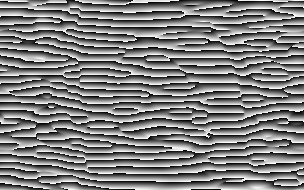
\includegraphics[trim = 100px 50px 110px 30px, clip, width=0.29\textwidth]{images/input/wrapped_harp.png}};
    \begin{scope}[x={(image.south east)},y={(image.north west)}]
        \draw[red,ultra thick] (0.5,0) -- (0.5,1);
    \end{scope}
\end{tikzpicture}
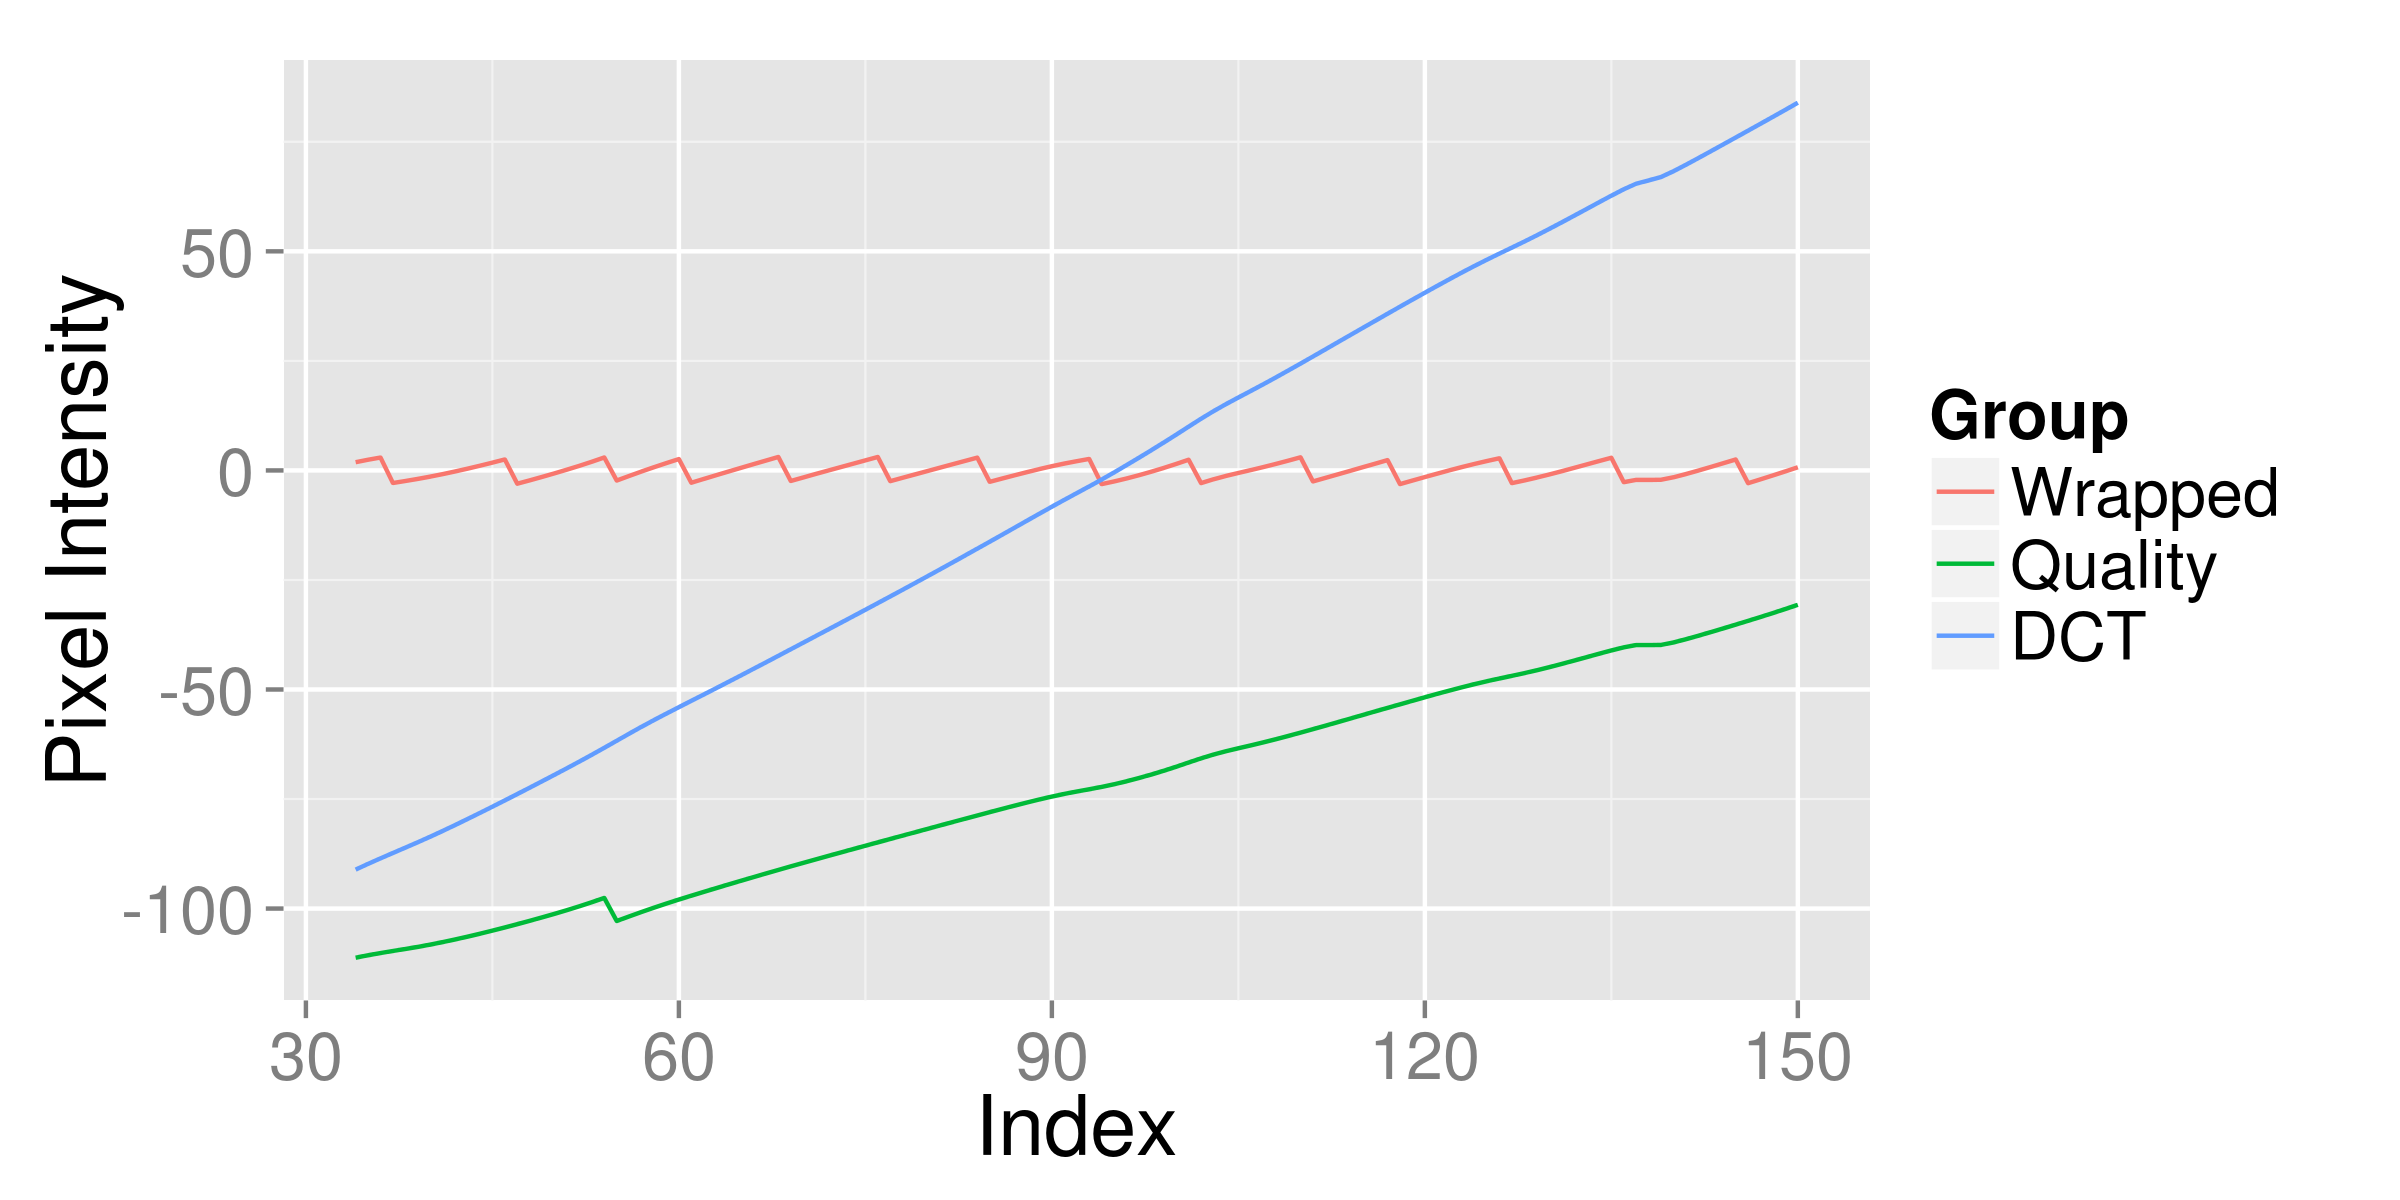
\includegraphics[width=0.70\textwidth]{images/harp/congruence.png}
\itkcaption[HARP_Congruence]{Congruence in HARP Data.  The pixel intensities from the vertical centerline of the HARP image are plotted for the unwrapped and original HARP data.  Note that the quality-guided approach is congruent throughout, but contains a discontinuity.  The DCT approach is smooth throughout, but is not congruent.}
\label{fig:HARP_Congruence}
\end{figure}

\subsection{A Note on Computational Speed}

The \code{itk::TimeProbe} class was used to measure the excecution time for the quality-guided and $L^2$-norm implementations on a single-processor Ubuntu 12.0.2 virtual machine with 4GB of memory.  For the SWI data, the quality-guided and $L^2$-norm approaches took $1.14$ and $0.75s$, respectively.  For the HARP data, the quality-guided and $L^2$-norm approaches took $0.40$ and $0.27s$, respectively.  Successive runs differed by less than 0.01s.  Therefore, the quality-guided approach took slighly less than twice as long to execute, though this difference may be insignificant for many applications.  Importantly, execution times are expected to grow linearly with input size for the quality-guided approach and by $O(n \log n)$ for the $L^2$-norm approach.  The quality-guided approach could be sped up by allowing for a mask that would prevent the unwrapping of pixels outside the area of interest and the DCT approach could be sped up by taking advantage of multithreading.  However, as has been shown, for some applications it may be necessary to incorporate the DCT algorithm into an iterative algorithm such as preconditioned conjugate gradient weighted $L^2$-norm in order to achieve satisfactory results, which could negate advantages gained through multithreading.